\begin{figure}[ht!]
    \centering
    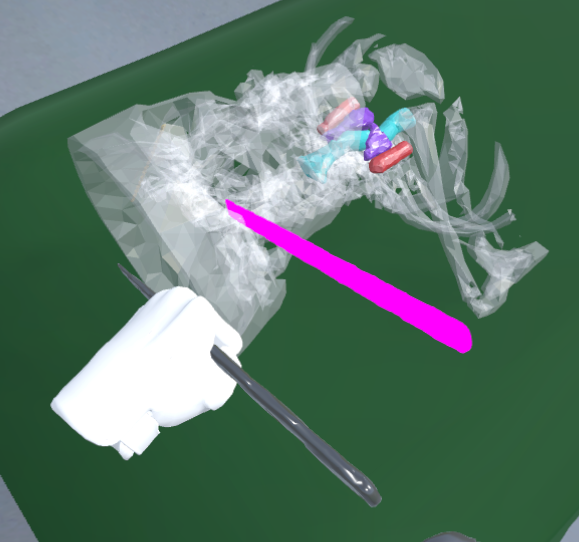
\includegraphics[width=\linewidth]{images/implementation/features/procedures/chisel.png}
    \caption{\label{fig::FeatureChisel}Hammer and Chisel Procedure}
\end{figure}

The chisel procedure has two parts to it.
First, with one hand, a chisel has to be chosen.
Users have a choice between a small, medium, large and extra large chisel to perform the procedure.
With the other hand, users then have to pick up the hammer.
By pressing the indicate button on the hand where the chisel is located, indications are shown to the user.
While these indications are active, the user has to "hammer" on these indications to perform the procedure \ref{fig::FeatureChisel}.
This will create a copy fo the currently hold chisel and add it to the project case.
The indicators are at the top and bottom end of each chisel, so that the user has to use a natural "hammering" motion to perform the procedure.